\section{Kontext- und Typeinschränkungen}
\label{sec:constraints}
In diesem Kapitel werden die nötigen Kontext Checks beschrieben.

\subsection{Kontext Einschränkungen}

Für conditions gilt grundsätzlich, dass bei ihrer Ausführung kein State verändert werden 
darf. In IML wurde dies durch die saubere Trennung von Expressions und Commands, sowie die standard
Kontext Checks bereits erreicht. Trotzdem sind einige weitere Einschränkungen nötig.

\begin{itemize}

\item Die Funktion old() darf nur innerhalb von postconditions aufgerufen werden.
\item Es darf keine weitere Funktion mit dem Namen old deklariert werden.
\item Das Label einer Condition muss innerhalb der Condition List einmalig sein.
\item Expressions innerhalb der Conditions müssen einen boolschen Wert erzeugen.

\end{itemize}

\subsubsection{Speicherzugriff}

\begin{itemize}
\item In Preconditions kann auf alle initialisierten Variablen und Konstanten zugegriffen werden, welche 
in der Parameterliste oder der Global Import List definiert wurden. Auf lokal deklarierte Variablen 
kann nicht zugegriffen werden. Da out-Parameter nicht initialisiert sind, stehen sie nicht zur
Verfügung.
\item In Postconditions kann auf alle Variablen und Konstanten zugegriffen werden, welche auch in 
Preconditions möglich sind. Zusätzlich sind alle lokal definierten Variablen und Konstanten verfügbar.
\item In Postconditions von Funktionen kann auf die Returnvariable zugegriffen werden.
\item In Postconditions von Prozeduren kann auf out-Parameter zugegriffen werden.
\item Die Funktion old() kann nicht auf Konstanten benutzt werden.
\item Die Funktion old() kann nur auf Variablen benutzt werden, welche in der Precondition verfügbar wären.

\end{itemize}

%\newpage

%\begin{figure*}[h]
%	\begin{center}
%		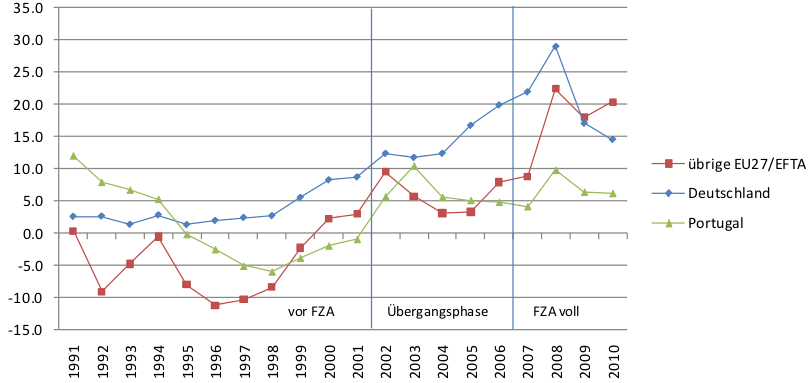
\includegraphics[width=0.9\textwidth]{images/Zuwanderungssaldo_Bericht_2.png}
%	\end{center}
%	\caption{Verlauf der Zuwanderung nach Herkunftsländern in Tausend \cite[S. 18]{ADMIN:Bericht}}
%	\label{fig:zuwanderungsaldi}
%\end{figure*}

